\documentclass[12pt,a4paper]{article}

\usepackage[utf8]{inputenc}
\usepackage[T1]{fontenc}
\usepackage{geometry}
\usepackage{graphicx}
\usepackage{float}
\usepackage{array}
\usepackage{booktabs}
\usepackage{longtable}
\usepackage{caption}
\usepackage{subcaption}
\usepackage{hyperref}
\usepackage{enumitem}
\usepackage{xcolor}
\usepackage{amsmath}
\usepackage{listings}

\geometry{margin=2.5cm}
\setlength{\parskip}{0.7em}
\setlength{\parindent}{0pt}
\renewcommand{\labelitemi}{--}
\renewcommand{\labelitemii}{--}
\captionsetup{font=small,labelfont=bf}
\hypersetup{
    colorlinks=true,
    linkcolor=blue!50!black,
    urlcolor=blue!60!black,
    pdftitle={Documentación del Proyecto - Organización Computacional},
    pdfauthor={Grupo 21}
}

\title{Documentación Técnica\\Proyecto - Organización Computacional}
\author{Grupo 21}
\date{29 de abril de 2026}

\begin{document}

\begin{titlepage}
    \centering
    \vspace*{1.5cm}
    
\includegraphics[width=0.23\textwidth]{assets/usac_logo.png}\par\vspace{1cm}
    {\scshape\LARGE Universidad de San Carlos de Guatemala \par}
    \vspace{0.4cm}
    {\scshape\Large Facultad de Ingeniería \par}
    \vspace{0.2cm}
    {\scshape\large Escuela de Ciencias y Sistemas \par}
    \vspace{1.8cm}
    {\Huge\bfseries Proyecto\\[0.2cm] Organización Computacional\par}
    \vspace{0.8cm}
    {\Large Documentación de la \textit{Casa Inteligente con Control de Ambientes y Ventilador Automatizado}\par}
    \vspace{1cm}
    \begin{tabular}{|c|p{8.2cm}|}
        \hline
        \textbf{Carnet} & \textbf{Integrante} \\
        \hline
        202406918 & Claudia Maribel Tigüilá Tecum \\
        \hline
        202403929 & Emiliana Elizabeth Pú Lara \\
        \hline
        202300476 & Alex Ricardo Castañeda Rodríguez \\
        \hline
        201904522 & Byron Manuel Hernández López \\
        \hline
    \end{tabular}
    \vfill
    {\large Grupo 21\par}
    {\large Abril de 2026\par}
    \vfill
\end{titlepage}

\tableofcontents
\newpage

\section{Resumen}
En este proyecto se desarrolló una maqueta de casa inteligente capaz de controlar cinco ambientes de iluminación, un ventilador DC y una puerta automatizada con servomotor. El sistema utiliza un Arduino como unidad central, memoria EEPROM para persistir escenas, una pantalla LCD I2C para retroalimentación local, una aplicación de escritorio para cargar configuraciones \texttt{.org} por USB y una aplicación móvil para activar modos por Bluetooth.

La solución cubre la lógica pedida en el PDF del proyecto: escenas persistentes, control remoto, validación de configuración, retroalimentación visual y documentación técnica del circuito, del flujo de datos y de los activos de software involucrados.

\section{Marco Formativo}

\subsection{Valor}
El proyecto integra conceptos de organización computacional con una implementación embebida real. La práctica de persistencia en EEPROM, comunicación serial, control de periféricos y organización modular del software permite aplicar teoría en un sistema funcional y verificable.

\subsection{Competencias}
Durante el desarrollo del proyecto se fortalecieron las siguientes competencias:
\begin{itemize}[leftmargin=1.2cm]
    \item Diseño e integración de sistemas embebidos con Arduino.
    \item Uso de memoria EEPROM para almacenamiento persistente.
    \item Definición y validación de formatos de entrada estructurados.
    \item Control de actuadores y salidas digitales desde una arquitectura centralizada.
    \item Desarrollo de interfaces de apoyo en escritorio y móvil.
    \item Documentación técnica de circuitos, flujo de datos y entregables.
\end{itemize}

\subsection{Objetivo SMART}
Diseñar, integrar y documentar antes del 2 de mayo de 2026 una maqueta funcional de casa inteligente con cinco ambientes, control de ventilador y puerta, escenas almacenadas en EEPROM, carga de configuración desde archivo \texttt{.org} y activación remota por Bluetooth, dejando evidencia del circuito, del código y del flujo completo de operación.

\section{Enunciado del Proyecto}

\subsection{Descripción del problema a resolver}
El proyecto plantea automatizar una vivienda a escala mediante escenas de iluminación predefinidas, persistencia de configuración y control remoto. El sistema debe permitir que un usuario defina modos desde una computadora por medio de un archivo \texttt{.org}, guarde esos modos en EEPROM, los active por Bluetooth o por serial y obtenga retroalimentación inmediata mediante LCD y LEDs de estado.

Además del control de luces, la solución incorpora un ventilador DC y una puerta automatizada con servomotor, con lo cual el sistema deja de ser solo un ejemplo de persistencia de datos y se convierte en una maqueta domótica funcional.

\subsection{Alcance del proyecto}
El repositorio cubre cuatro bloques principales:
\begin{itemize}[leftmargin=1.2cm]
    \item El sketch de Arduino que implementa persistencia, lectura de comandos, control de LEDs, ventilador, LCD y puerta.
    \item La aplicación de escritorio \texttt{EEPROM\_Liquid\_Controller}, usada para seleccionar y enviar archivos \texttt{.org} por USB.
    \item La aplicación móvil \texttt{eeprom\_liquid\_remote}, usada para activar modos desde Bluetooth clásico.
    \item Los diagramas y evidencias visuales del montaje y de las interfaces del sistema.
\end{itemize}

\section{Requisitos Funcionales}
Con base en el PDF del proyecto, los requisitos funcionales principales atendidos por la solución son los siguientes:

\subsection{Control de escenas}
\begin{itemize}[leftmargin=1.2cm]
    \item \texttt{modo\_fiesta}
    \item \texttt{modo\_relajado}
    \item \texttt{modo\_noche}
    \item \texttt{encender\_todo}
    \item \texttt{apagar\_todo}
\end{itemize}

Cada escena almacena estado del ventilador, patrón de LEDs y mensaje para LCD.

\subsection{Persistencia en EEPROM}
Cada escena se guarda en una dirección fija de EEPROM mediante una estructura con los siguientes campos:
\begin{itemize}[leftmargin=1.2cm]
    \item \texttt{magic}
    \item \texttt{fan}
    \item \texttt{ledPattern}
    \item \texttt{message[33]}
\end{itemize}

El sistema además precarga modos por defecto si no detecta una configuración válida.

\subsection{Carga de configuración desde archivo \texttt{.org}}
El sketch reconoce el flujo:
\begin{enumerate}
    \item \texttt{conf\_ini}
    \item Definición de uno o varios modos
    \item \texttt{conf:fin}
\end{enumerate}

Durante la carga:
\begin{itemize}[leftmargin=1.2cm]
    \item Se ignoran líneas vacías y comentarios con \texttt{//}.
    \item Se valida que cada modo tenga ventilador y patrón de LEDs.
    \item Si hay error de sintaxis, se cancela la carga y se reporta \texttt{UPLOAD\_ERROR}.
    \item Si la carga finaliza correctamente, el LED verde parpadea tres veces y el LCD muestra confirmación.
\end{itemize}

\subsection{Control remoto por Bluetooth y serial}
Comandos soportados por el sketch:
\begin{itemize}[leftmargin=1.2cm]
    \item \texttt{modo\_fiesta}
    \item \texttt{modo\_relajado}
    \item \texttt{modo\_noche}
    \item \texttt{encender\_todo}
    \item \texttt{apagar\_todo}
    \item \texttt{estado}
    \item \texttt{abrir\_puerta}
    \item \texttt{cerrar\_puerta}
\end{itemize}

\subsection{Retroalimentación local}
\begin{itemize}[leftmargin=1.2cm]
    \item LCD I2C 16x2 con mensaje del modo y estado del ventilador.
    \item LED azul para sistema listo.
    \item LED verde para carga exitosa.
    \item LED rojo para errores.
\end{itemize}

\subsection{Actuadores y salidas}
\begin{itemize}[leftmargin=1.2cm]
    \item Cinco salidas de iluminación: sala, comedor, cocina, baño y habitación.
    \item Un motor DC para ventilador.
    \item Un servomotor para apertura y cierre de puerta.
    \item Un botón físico con \textit{debounce} para alternar la puerta.
\end{itemize}

\section{Arquitectura de la Solución}

\subsection{Descripción general}
La arquitectura se divide en tres capas operativas:
\begin{enumerate}
    \item Unidad central Arduino: recibe comandos por serial, administra EEPROM y controla salidas físicas.
    \item Interfaz de escritorio: prepara y transmite archivos \texttt{.org} al Arduino por USB.
    \item Interfaz móvil: envía comandos por Bluetooth clásico para activar modos o consultar estado.
\end{enumerate}

\begin{table}[H]
    \centering
    \caption{Flujo general del sistema.}
    \begin{tabular}{p{5.5cm}p{8cm}}
        \toprule
        \textbf{Origen} & \textbf{Destino y función} \\
        \midrule
        Archivo \texttt{.org} & App de escritorio $\rightarrow$ Serial USB $\rightarrow$ Arduino $\rightarrow$ EEPROM \\
        Teléfono Android & Bluetooth HC-06 $\rightarrow$ Arduino $\rightarrow$ luces, LCD, ventilador y puerta \\
        EEPROM & Arduino $\rightarrow$ recuperación y aplicación del modo activo \\
        \bottomrule
    \end{tabular}
\end{table}

\subsection{Unidad central de procesamiento}
El archivo principal del sistema es \texttt{arduino/eeprom\_liquid\_controller/eeprom\_liquid\_controller.ino}. En él se definen los pines, el protocolo de carga del archivo \texttt{.org}, el mapa de EEPROM, la gestión de escenas y el control de actuadores.

\begin{table}[H]
    \centering
    \caption{Distribución de pines según el sketch.}
    \begin{tabular}{c p{9.5cm}}
        \toprule
        \textbf{Pin} & \textbf{Uso} \\
        \midrule
        0 & \texttt{rx\_bluetooth} \\
        1 & \texttt{tx\_bluetooth} \\
        2 & \texttt{led\_azul} \\
        3 & \texttt{led\_verde} \\
        4 & \texttt{led\_rojo} \\
        5 & \texttt{luces\_sala} \\
        6 & \texttt{luces\_comedor} \\
        7 & \texttt{luces\_cocina} \\
        8 & \texttt{luces\_bano} \\
        9 & \texttt{servo\_puerta} \\
        10 & \texttt{motor\_ventilador} \\
        11 & \texttt{boton\_puerta} \\
        12 & \texttt{luces\_habitacion} \\
        A4 & SDA del LCD I2C \\
        A5 & SCL del LCD I2C \\
        \bottomrule
    \end{tabular}
\end{table}

La tabla anterior corresponde de forma directa con las constantes definidas en el sketch. Esto permite relacionar el diagrama en Proteus con la implementación real y comprobar que cada bloque mostrado en la documentación sí tiene una salida física asociada en el Arduino.

\begin{figure}[H]
    \centering
    \begin{minipage}{0.9\textwidth}
        \begin{lstlisting}[basicstyle=\ttfamily\footnotesize]
const int led_azul = 2;
const int led_verde = 3;
const int led_rojo = 4;
const int luces_sala = 5;
const int luces_comedor = 6;
const int luces_cocina = 7;
const int luces_bano = 8;
const int servo_puerta = 9;
const int motor_ventilador = 10;
const int boton_puerta = 11;
const int luces_habitacion = 12;
        \end{lstlisting}
    \end{minipage}
    \caption{Definición de pines usada por el sketch Arduino.}
\end{figure}

\subsection{Apps de apoyo}
\begin{table}[H]
    \centering
    \caption{Bloques de software del repositorio.}
    \small
    \begin{tabular}{>{\raggedright\arraybackslash}p{3.5cm} >{\raggedright\arraybackslash}p{3.3cm} >{\raggedright\arraybackslash}p{6.4cm}}
        \toprule
        \textbf{Componente} & \textbf{Tecnología} & \textbf{Función} \\
        \midrule
        \texttt{EEPROM\_Liquid\_\newline Controller} & Python + Tkinter & Selección de puerto, carga de archivo \texttt{.org} y envío serial \\
        \texttt{eeprom\_liquid\_remote} & Flutter & Conexión Bluetooth y envío de comandos de modo \\
        Sketch Arduino & C++ para Arduino & Procesamiento central, EEPROM, LCD, luces, ventilador y puerta \\
        \bottomrule
    \end{tabular}
\end{table}

Las aplicaciones de apoyo sirven para cargar configuraciones y enviar comandos. La lógica del sistema sigue concentrada en el Arduino: allí se validan escenas, se escriben datos en EEPROM y se activan luces, ventilador y puerta.

\section{Formato del archivo \texttt{.org}}

\subsection{Sintaxis reconocida por el sketch}
Las reglas observadas en el sketch son las siguientes:
\begin{itemize}[leftmargin=1.2cm]
    \item El archivo debe iniciar con \texttt{conf\_ini}.
    \item Debe cerrar con \texttt{conf:fin}.
    \item Los comentarios usan \texttt{//}.
    \item Cada modo se define por su nombre.
    \item Para cada modo deben declararse \texttt{Ventilador:} y \texttt{LED'S:}.
    \item \texttt{Mensaje en LCD:} es opcional; si no aparece, el sistema usa un mensaje por defecto.
\end{itemize}

La validación se hace durante la lectura serial, línea por línea. Así, cuando aparece un error, el sistema puede marcarlo enseguida en el LCD, en el LED rojo y en la salida serial.

\begin{figure}[H]
    \centering
    \begin{minipage}{0.9\textwidth}
        \begin{lstlisting}[basicstyle=\ttfamily\footnotesize]
void processLine(String rawLine) {
  String line = stripComment(rawLine);
  line.trim();
  if (line.length() == 0) return;

  if (line == "conf_ini") {
    beginUpload();
    return;
  }

  if (uploadActive) {
    processUploadLine(line);
    return;
  }

  processCommand(line);
}
        \end{lstlisting}
    \end{minipage}
    \caption{Separación entre modo de carga y modo de comandos en el sketch.}
\end{figure}

\subsection{Valores válidos}
\begin{table}[H]
    \centering
    \caption{Valores reconocidos por el formato \texttt{.org}.}
    \begin{tabular}{p{4cm}p{8cm}}
        \toprule
        \textbf{Campo} & \textbf{Valores válidos} \\
        \midrule
        Modo & \texttt{modo\_fiesta}, \texttt{modo\_relajado}, \texttt{modo\_noche}, \texttt{encender\_todo}, \texttt{apagar\_todo} \\
        Ventilador & \texttt{ON}, \texttt{OFF} \\
        LEDs & \texttt{ON}, \texttt{OFF}, \texttt{Alternandose} \\
        \bottomrule
    \end{tabular}
\end{table}

\subsection{Ejemplo completo}
\begin{figure}[H]
    \centering
    \fbox{
        \parbox{0.9\textwidth}{
        \ttfamily
        // Configuracion de modos para el sistema de control\\
        conf\_ini\\
        \\
        modo\_fiesta\\
        Mensaje en LCD: "Modo: FIESTA."\\
        Ventilador: ON\\
        LED'S: Alternandose\\
        \\
        modo\_relajado\\
        Mensaje en LCD: "Modo: RELAJADO."\\
        Ventilador: OFF\\
        LED'S: ON\\
        \\
        modo\_noche\\
        Mensaje en LCD: "Modo: NOCHE."\\
        Ventilador: OFF\\
        LED'S: OFF\\
        \\
        encender\_todo\\
        Mensaje en LCD: "Modo: TODO ON."\\
        Ventilador: ON\\
        LED'S: ON\\
        \\
        apagar\_todo\\
        Mensaje en LCD: "Modo: TODO OFF."\\
        Ventilador: OFF\\
        LED'S: OFF\\
        \\
        conf:fin
        }
    }
    \caption{Ejemplo de archivo \texttt{.org} compatible con el sistema.}
\end{figure}

\subsection{Errores detectados}
El sketch cancela la carga si detecta:
\begin{itemize}[leftmargin=1.2cm]
    \item modo no definido
    \item modo incompleto
    \item línea inválida
    \item ventilador inválido
    \item LEDs inválidos
    \item archivo vacío
\end{itemize}

Si aparece uno de estos fallos, la carga se detiene y el sistema muestra el motivo tanto en pantalla como por serial.

\begin{figure}[H]
    \centering
    \begin{minipage}{0.9\textwidth}
        \begin{lstlisting}[basicstyle=\ttfamily\footnotesize]
void failUpload(const char *reason) {
  uploadActive = false;
  currentUploadMode = NO_MODE;
  systemError = true;
  digitalWrite(led_azul, LOW);
  digitalWrite(led_verde, LOW);
  digitalWrite(led_rojo, HIGH);
  showLcd("Error archivo", reason);
  Serial.print("UPLOAD_ERROR:");
  Serial.println(reason);
}
        \end{lstlisting}
    \end{minipage}
    \caption{Rutina de error durante la carga del archivo \texttt{.org}.}
\end{figure}

\section{Tabla de direcciones EEPROM}
La EEPROM quedó definida con direcciones fijas por modo. Cada escena inicia en una posición constante y desde allí se escribe la estructura completa de 36 bytes: 1 byte para \texttt{magic}, 1 byte para \texttt{fan}, 1 byte para \texttt{ledPattern} y 33 bytes para \texttt{message}.

\begin{table}[H]
    \centering
    \caption{Direcciones fijas de almacenamiento de escenas en EEPROM.}
    \small
    \begin{tabular}{p{3.2cm}c p{7.8cm}}
        \toprule
        \textbf{Modo} & \textbf{Dirección fija} & \textbf{Valores por defecto} \\
        \midrule
        \texttt{modo\_fiesta} & 0 & Ventilador ON, LEDs Alternandose, mensaje \texttt{Modo: FIESTA.} \\
        \texttt{modo\_relajado} & 36 & Ventilador OFF, LEDs ON, mensaje \texttt{Modo: RELAJADO.} \\
        \texttt{modo\_noche} & 72 & Ventilador OFF, LEDs OFF, mensaje \texttt{Modo: NOCHE.} \\
        \texttt{encender\_todo} & 108 & Ventilador ON, LEDs ON, mensaje \texttt{Modo: TODO ON.} \\
        \texttt{apagar\_todo} & 144 & Ventilador OFF, LEDs OFF, mensaje \texttt{Modo: TODO OFF.} \\
        \bottomrule
    \end{tabular}
\end{table}

Estas direcciones están definidas de forma literal en el sketch. Por eso aquí se toman como posiciones fijas:

\begin{figure}[H]
    \centering
    \begin{minipage}{0.9\textwidth}
        \begin{lstlisting}[basicstyle=\ttfamily\footnotesize]
const int EEPROM_ADDR_FIESTA = 0;
const int EEPROM_ADDR_RELAJADO = 36;
const int EEPROM_ADDR_NOCHE = 72;
const int EEPROM_ADDR_ENCENDER_TODO = 108;
const int EEPROM_ADDR_APAGAR_TODO = 144;
        \end{lstlisting}
    \end{minipage}
    \caption{Definición explícita de direcciones fijas en EEPROM.}
\end{figure}

La escritura persistente también se hace sobre esas posiciones mediante \texttt{EEPROM.put()}, usando la estructura \texttt{SceneConfig}. Así, cada modo conserva su configuración incluso después de reiniciar el Arduino.

\begin{figure}[H]
    \centering
    \begin{minipage}{0.9\textwidth}
        \begin{lstlisting}[basicstyle=\ttfamily\footnotesize]
void writeSceneToEeprom(byte mode, PendingScene scene) {
  SceneConfig stored;
  stored.magic = EEPROM_MAGIC;
  stored.fan = scene.fan;
  stored.ledPattern = scene.ledPattern;
  copyMessage(String(scene.message), stored.message);
  EEPROM.put(eepromAddress(mode), stored);
}
        \end{lstlisting}
    \end{minipage}
    \caption{Rutina de escritura de escenas en EEPROM.}
\end{figure}

\section{Implementación Física}

\subsection{Diagrama general y esquema}
La vista general ordena el proyecto por módulos. Arriba están los bloques de control y monitoreo; abajo, las salidas físicas de la casa. Sirve para ver de un golpe cómo se conectan Arduino, Bluetooth, LCD, iluminación, ventilación y puerta.

\begin{figure}[H]
    \centering
    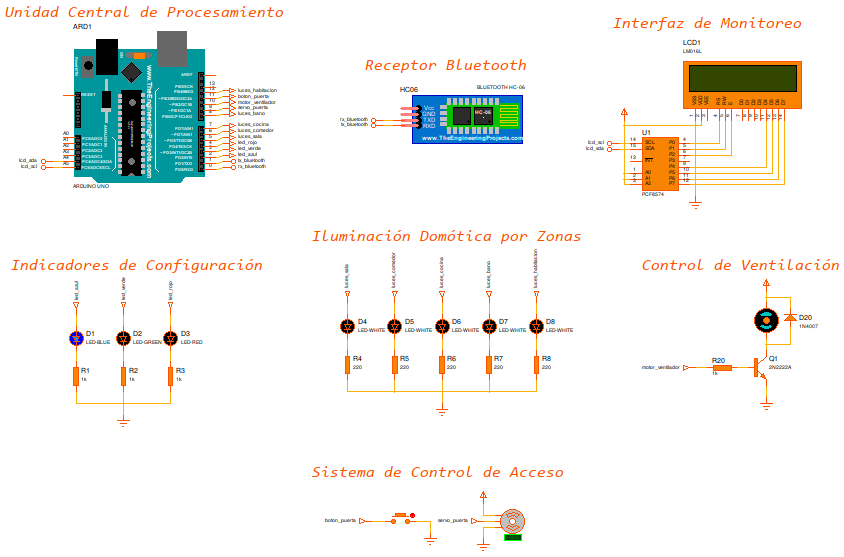
\includegraphics[width=\textwidth]{assets/proteus_vista_general.png}
    \caption{Vista modular general del sistema.}
\end{figure}

\subsection{Unidad central y periféricos}
La unidad central mostrada en Proteus corresponde al bloque que arranca el sistema. Desde aquí se configuran pines, se habilita la comunicación serial, se conecta el servomotor, se inicializa el LCD y se cargan escenas por defecto si la EEPROM aún no tiene datos válidos.

\begin{figure}[H]
    \centering
    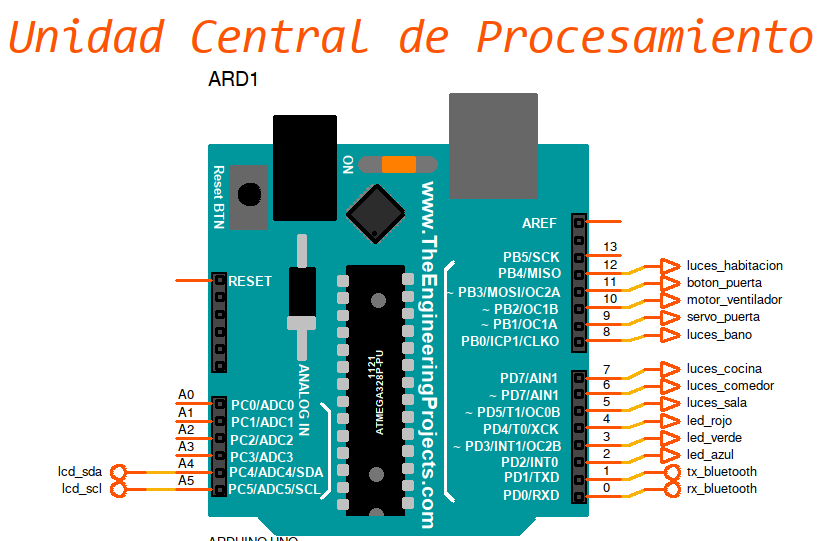
\includegraphics[width=0.85\textwidth]{assets/proteus_arduino_unidad_central.png}
    \caption{Unidad central de procesamiento basada en Arduino.}
\end{figure}

\begin{figure}[H]
    \centering
    \begin{minipage}{0.9\textwidth}
        \begin{lstlisting}[basicstyle=\ttfamily\footnotesize]
void setup() {
  Serial.begin(BAUDRATE);
  doorServo.attach(servo_puerta);
  closeDoor();
  lcd.init();
  lcd.backlight();
  setReadyState();
  seedDefaultScenesIfNeeded();
  applyMode(MODE_APAGAR_TODO);
}
        \end{lstlisting}
    \end{minipage}
    \caption{Secuencia principal de inicialización del sistema.}
\end{figure}

El receptor HC-06 es el canal de control remoto. Por aquí llegan textos como \texttt{modo\_fiesta}, \texttt{modo\_noche} o \texttt{estado}. El sketch los procesa igual que si vinieran del monitor serial.

\begin{figure}[H]
    \centering
    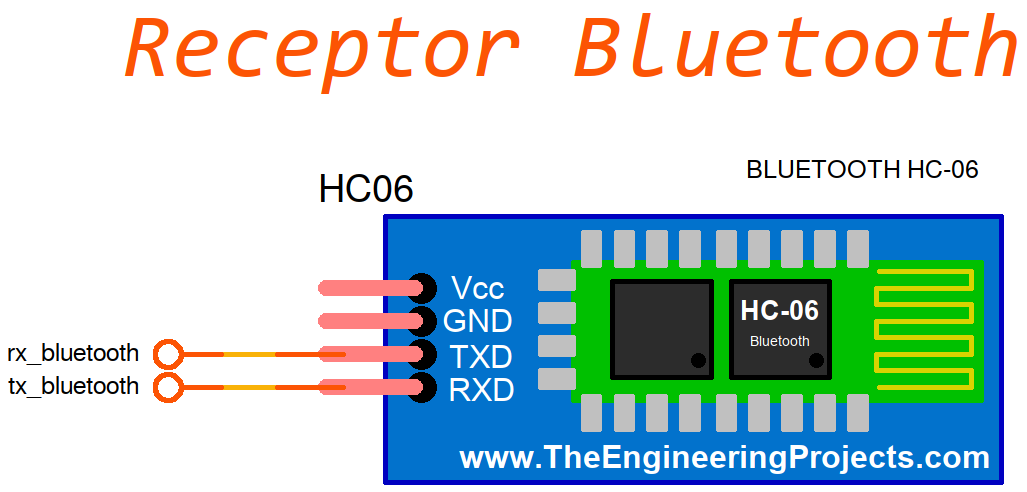
\includegraphics[width=0.85\textwidth]{assets/proteus_bluetooth_hc06.png}
    \caption{Receptor Bluetooth HC-06.}
\end{figure}

La pantalla LCD se usa para mostrar el estado del sistema. El Arduino la actualiza cada vez que cambia de modo o detecta un problema de configuración.

\begin{figure}[H]
    \centering
    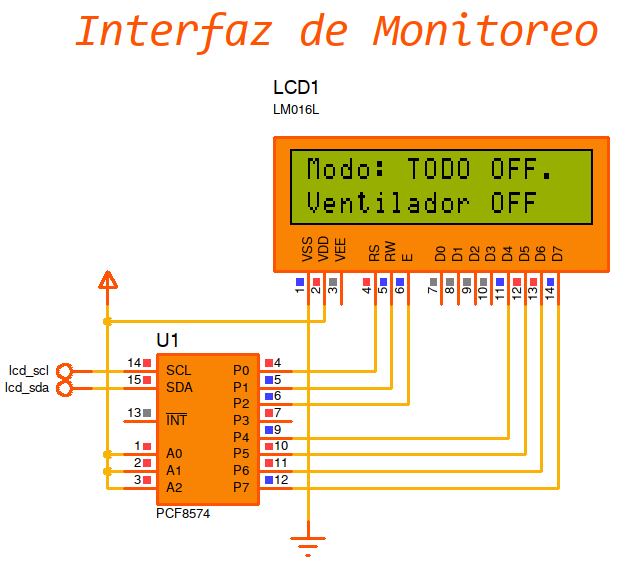
\includegraphics[width=0.75\textwidth]{assets/proteus_lcd_i2c.png}
    \caption{Interfaz de monitoreo con LCD I2C.}
\end{figure}

\begin{figure}[H]
    \centering
    \begin{minipage}{0.9\textwidth}
        \begin{lstlisting}[basicstyle=\ttfamily\footnotesize]
showLcd(scene.message,
        scene.fan == FAN_ON ? "Ventilador ON"
                            : "Ventilador OFF");
        \end{lstlisting}
    \end{minipage}
    \caption{Actualización del LCD al aplicar una escena.}
\end{figure}

\subsection{Módulos de salida}
El bloque de indicadores resume tres estados del sistema: azul para listo, verde para carga exitosa y rojo para error. Estas salidas coinciden con las rutinas \texttt{setReadyState()}, \texttt{blinkGreenSuccess()} y \texttt{failUpload()} del sketch.

\begin{figure}[H]
    \centering
    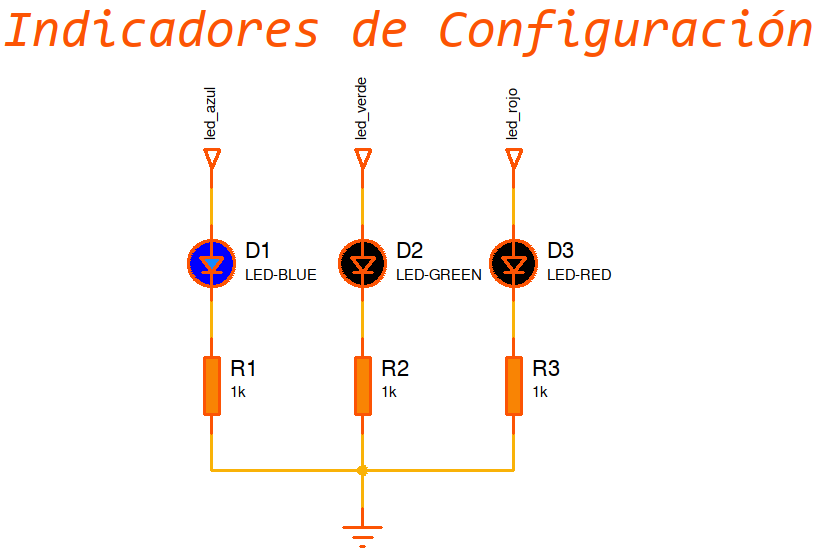
\includegraphics[width=0.75\textwidth]{assets/proteus_leds_estado.png}
    \caption{Indicadores de configuración.}
\end{figure}

La iluminación por zonas representa cinco salidas independientes: sala, comedor, cocina, baño y habitación. El proyecto no trabaja con un único LED general, sino con un conjunto de ambientes que pueden quedar todos encendidos, todos apagados o alternándose en el modo fiesta.

\begin{figure}[H]
    \centering
    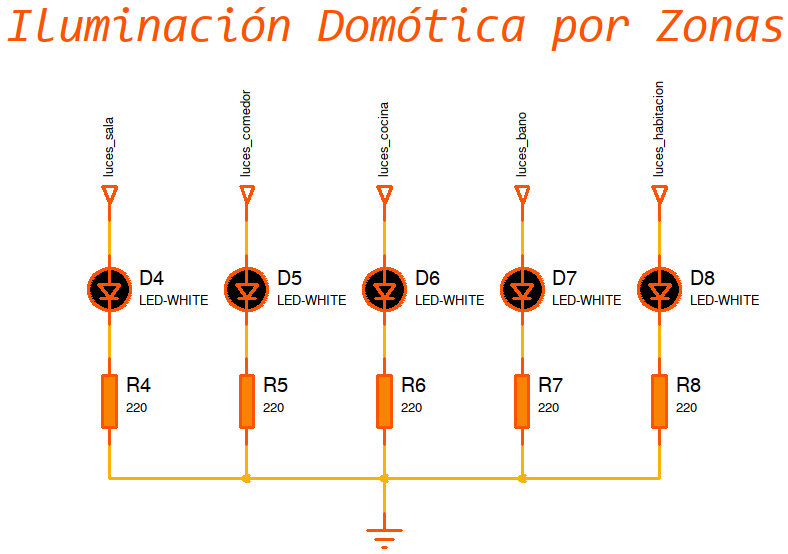
\includegraphics[width=0.75\textwidth]{assets/proteus_iluminacion_zonas.png}
    \caption{Iluminación domótica por zonas.}
\end{figure}

\begin{figure}[H]
    \centering
    \begin{minipage}{0.9\textwidth}
        \begin{lstlisting}[basicstyle=\ttfamily\footnotesize]
void setAllRoomLights(byte state) {
  digitalWrite(luces_sala, state);
  digitalWrite(luces_comedor, state);
  digitalWrite(luces_cocina, state);
  digitalWrite(luces_bano, state);
  digitalWrite(luces_habitacion, state);
}
        \end{lstlisting}
    \end{minipage}
    \caption{Rutina que controla simultáneamente los cinco ambientes.}
\end{figure}

En el modo fiesta, el sketch no deja todas las luces fijas; las alterna usando \texttt{millis()}. Por eso este bloque no se queda en una conexión de LEDs, sino que responde a un patrón temporal real.

\begin{figure}[H]
    \centering
    \begin{minipage}{0.9\textwidth}
        \begin{lstlisting}[basicstyle=\ttfamily\footnotesize]
if (now - lastAlternateTick < 450) return;
lastAlternateTick = now;
alternatePhase = !alternatePhase;
digitalWrite(luces_sala, alternatePhase ? HIGH : LOW);
digitalWrite(luces_comedor, alternatePhase ? LOW : HIGH);
digitalWrite(luces_cocina, alternatePhase ? HIGH : LOW);
digitalWrite(luces_bano, alternatePhase ? LOW : HIGH);
digitalWrite(luces_habitacion, alternatePhase ? HIGH : LOW);
        \end{lstlisting}
    \end{minipage}
    \caption{Patrón alternado de LEDs usado para \texttt{modo\_fiesta}.}
\end{figure}

El módulo de ventilación se controla como una salida digital simple. El Arduino solo decide si el ventilador está encendido o apagado según lo guardado en la escena activa.

\begin{figure}[H]
    \centering
    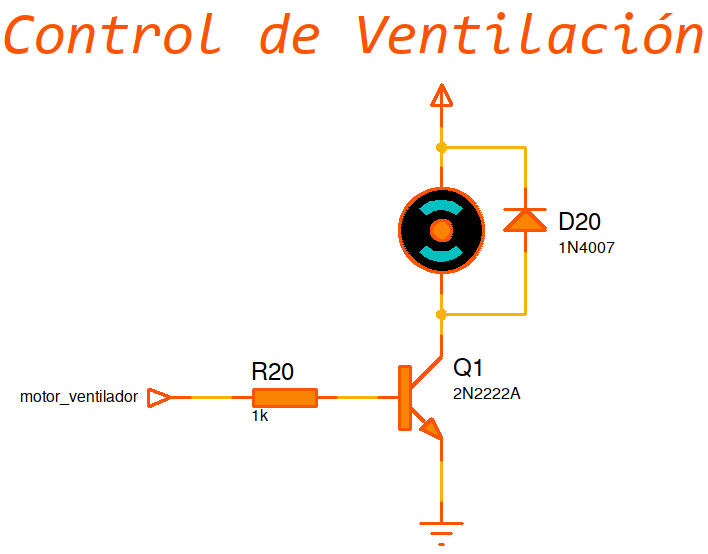
\includegraphics[width=0.75\textwidth]{assets/proteus_control_ventilador.png}
    \caption{Control de ventilación con motor DC.}
\end{figure}

\begin{figure}[H]
    \centering
    \begin{minipage}{0.9\textwidth}
        \begin{lstlisting}[basicstyle=\ttfamily\footnotesize]
digitalWrite(motor_ventilador,
             scene.fan == FAN_ON ? HIGH : LOW);
        \end{lstlisting}
    \end{minipage}
    \caption{Activación directa del ventilador desde la escena actual.}
\end{figure}

El sistema de control de acceso muestra la parte mecánica de la puerta. En el sketch, el botón físico conectado al pin 11 pasa por una lógica de antirrebote y luego alterna entre abrir y cerrar.

\begin{figure}[H]
    \centering
    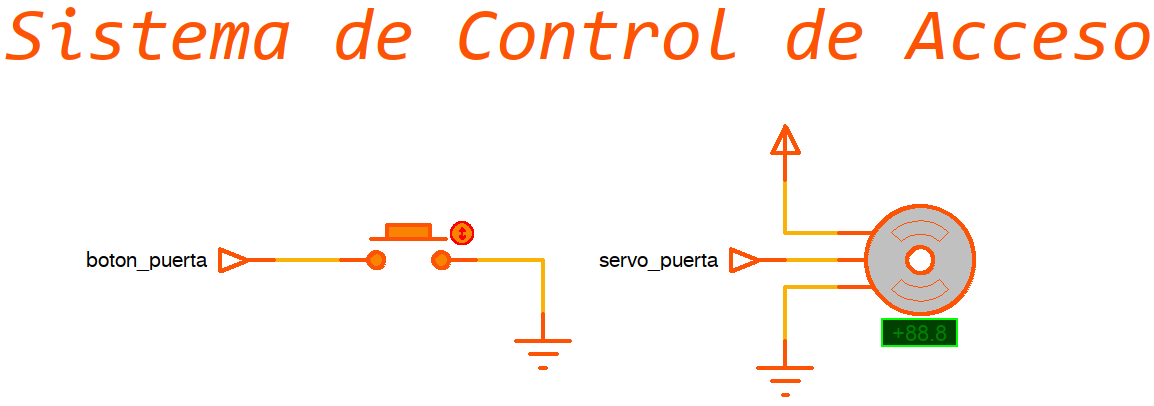
\includegraphics[width=0.65\textwidth]{assets/proteus_control_puerta.png}
    \caption{Sistema de control de acceso para la puerta.}
\end{figure}

\begin{figure}[H]
    \centering
    \begin{minipage}{0.9\textwidth}
        \begin{lstlisting}[basicstyle=\ttfamily\footnotesize]
if ((millis() - lastDoorDebounce) > 40) {
  if (reading != stableDoorButtonState) {
    stableDoorButtonState = reading;
    if (stableDoorButtonState == LOW) {
      if (doorOpen) closeDoor();
      else openDoor();
    }
  }
}
        \end{lstlisting}
    \end{minipage}
    \caption{Lógica de antirrebote y alternancia usada para la puerta.}
\end{figure}

\subsection{Interfaces del sistema}
La pantalla inicial de la aplicación de escritorio es el punto de entrada para cargar escenas persistentes. Desde aquí el usuario selecciona puerto, prepara el archivo y lo envía al Arduino.

\begin{figure}[H]
    \centering
    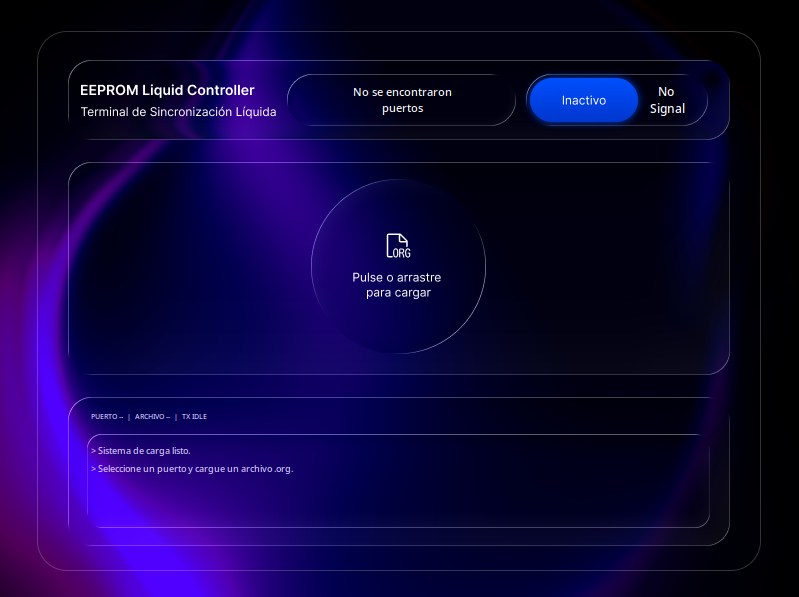
\includegraphics[width=\textwidth]{assets/app_escritorio_inicio.png}
    \caption{Pantalla inicial de la aplicación de escritorio.}
\end{figure}

La segunda captura muestra el archivo ya cargado en la interfaz. El contenido \texttt{.org} se trabaja como texto editable y visible antes de llegar al Arduino.

\begin{figure}[H]
    \centering
    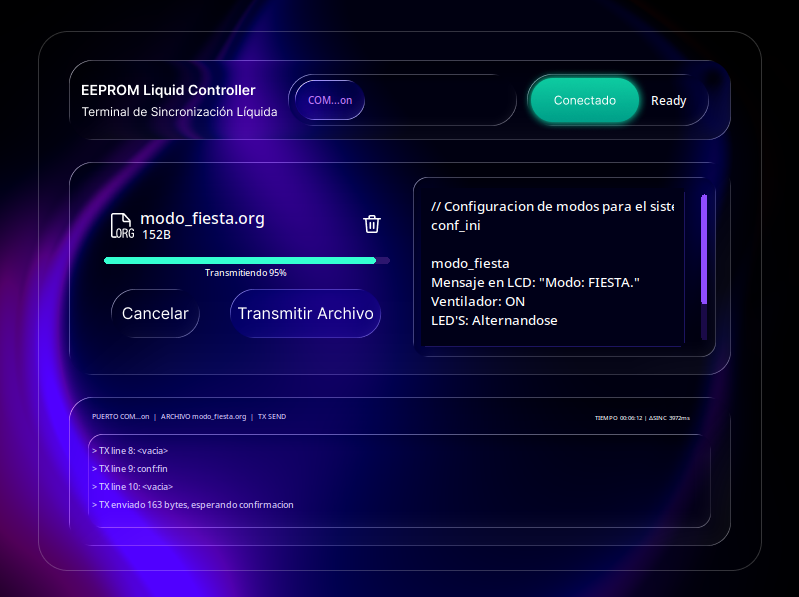
\includegraphics[width=\textwidth]{assets/app_escritorio_archivo_cargado.png}
    \caption{Archivo cargado en la aplicación de escritorio.}
\end{figure}

La tercera captura corresponde a la fase de transferencia. En ese punto el Arduino ya dejó de interpretar entradas como comandos normales y las procesa como líneas de configuración.

\begin{figure}[H]
    \centering
    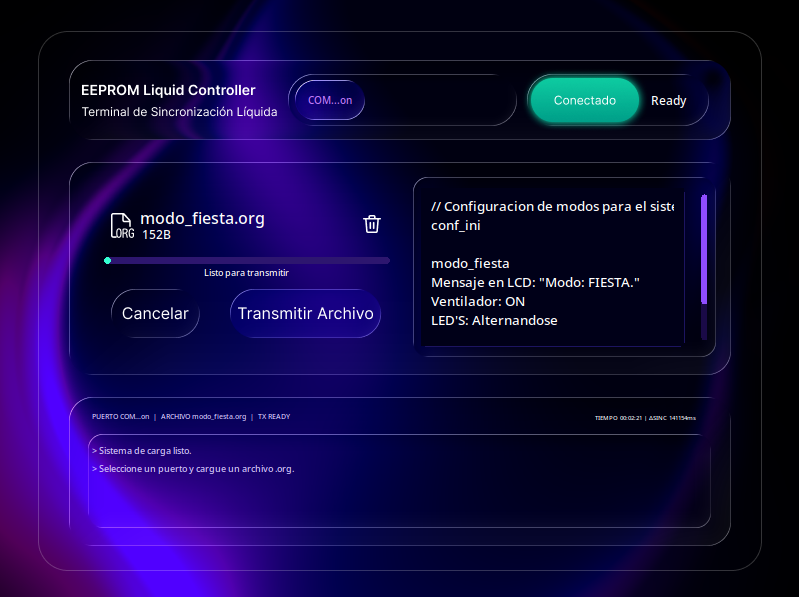
\includegraphics[width=\textwidth]{assets/app_escritorio_transferencia.png}
    \caption{Transferencia activa del archivo \texttt{.org}.}
\end{figure}

La aplicación móvil se muestra en dos pasos porque el flujo real tiene dos fases: primero seleccionar el dispositivo Bluetooth correcto y luego enviar acciones concretas. El sketch solo necesita recibir cadenas como \texttt{modo\_fiesta}, \texttt{modo\_noche} o \texttt{estado}.

\begin{figure}[H]
    \centering
    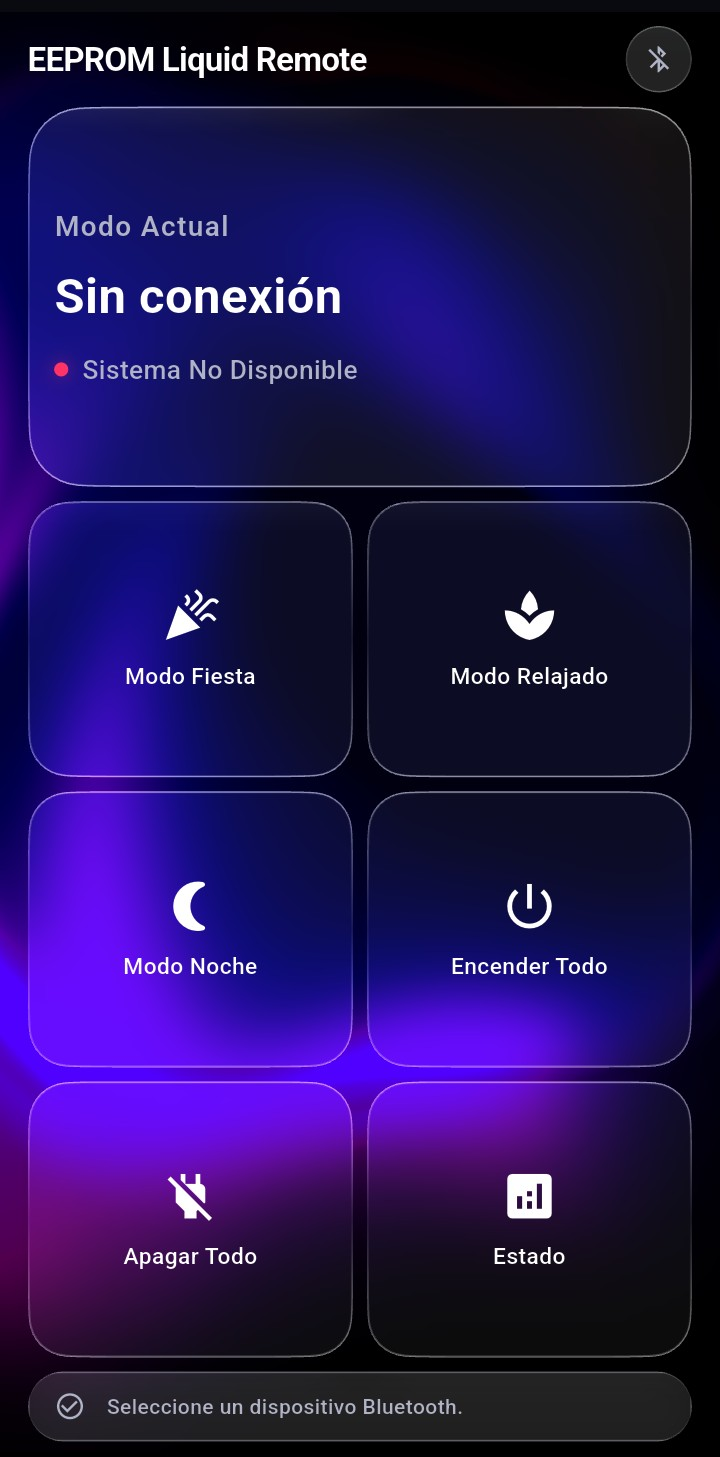
\includegraphics[width=0.42\textwidth]{assets/app_movil_panel_principal.jpeg}
    \caption{Panel principal de la aplicación móvil.}
\end{figure}

\begin{figure}[H]
    \centering
    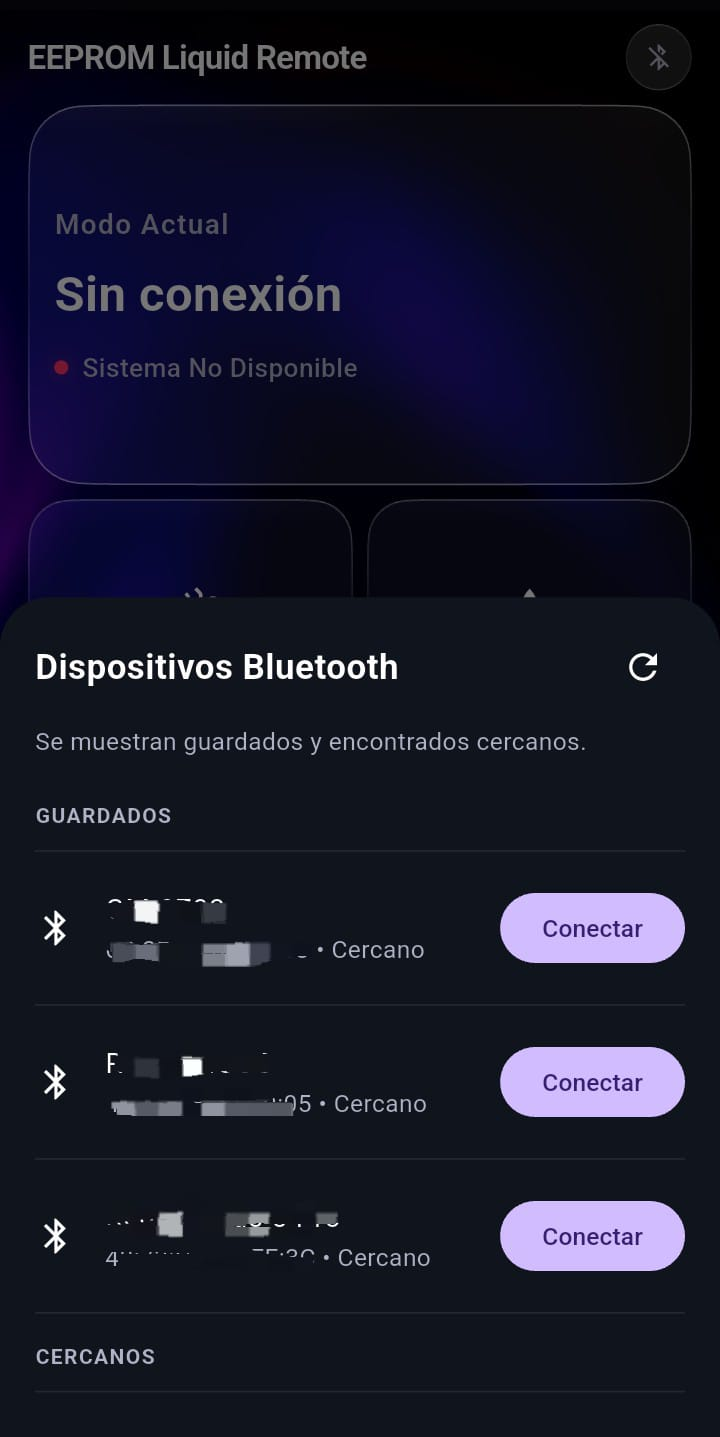
\includegraphics[width=0.42\textwidth]{assets/app_movil_dispositivos_bluetooth.jpeg}
    \caption{Pantalla de dispositivos Bluetooth de la aplicación móvil.}
\end{figure}

\section{Fragmentos clave del código Arduino}
Esta sección reúne los bloques del sketch que gobiernan el comportamiento general del sistema.

\subsection{Aplicación de escenas}
La rutina \texttt{applyMode()} enlaza EEPROM, LEDs de estado, LCD, ventilador e iluminación. Primero valida que la escena leída tenga firma correcta, luego actualiza el estado general del sistema y finalmente activa las salidas físicas.

\begin{figure}[H]
    \centering
    \begin{minipage}{0.9\textwidth}
        \begin{lstlisting}[basicstyle=\ttfamily\footnotesize]
void applyMode(byte mode) {
  SceneConfig scene = readSceneFromEeprom(mode);
  if (scene.magic != EEPROM_MAGIC) {
    systemError = true;
    digitalWrite(led_rojo, HIGH);
    showLcd("Modo sin config", modeName(mode));
    return;
  }

  activeMode = mode;
  systemError = false;
  digitalWrite(led_rojo, LOW);
  digitalWrite(led_azul, HIGH);
  digitalWrite(motor_ventilador, scene.fan == FAN_ON ? HIGH : LOW);
  applyLedPattern(scene.ledPattern);
  showLcd(scene.message,
          scene.fan == FAN_ON ? "Ventilador ON" : "Ventilador OFF");
}
        \end{lstlisting}
    \end{minipage}
    \caption{Rutina principal de aplicación de una escena almacenada.}
\end{figure}

\subsection{Escenas por defecto}
El proyecto no depende exclusivamente de una carga manual inicial. Si la EEPROM todavía no contiene una configuración válida, el Arduino crea escenas base para que la maqueta pueda arrancar operativa.

\begin{figure}[H]
    \centering
    \begin{minipage}{0.9\textwidth}
        \begin{lstlisting}[basicstyle=\ttfamily\footnotesize]
void seedDefaultScenesIfNeeded() {
  SceneConfig first = readSceneFromEeprom(MODE_APAGAR_TODO);
  if (first.magic == EEPROM_MAGIC) return;

  writeDefaultScene(MODE_FIESTA, FAN_ON, LEDS_ALTERNATING, "Modo: FIESTA.");
  writeDefaultScene(MODE_RELAJADO, FAN_OFF, LEDS_ON, "Modo: RELAJADO.");
  writeDefaultScene(MODE_NOCHE, FAN_OFF, LEDS_OFF, "Modo: NOCHE.");
  writeDefaultScene(MODE_ENCENDER_TODO, FAN_ON, LEDS_ON, "Modo: TODO ON.");
  writeDefaultScene(MODE_APAGAR_TODO, FAN_OFF, LEDS_OFF, "Modo: TODO OFF.");
}
        \end{lstlisting}
    \end{minipage}
    \caption{Inicialización automática de escenas por defecto.}
\end{figure}

\subsection{Comandos operativos}
Además de aplicar modos, el sketch soporta comandos puntuales que no requieren recargar la configuración completa, por ejemplo consultar estado o controlar la puerta de forma directa.

\begin{figure}[H]
    \centering
    \begin{minipage}{0.9\textwidth}
        \begin{lstlisting}[basicstyle=\ttfamily\footnotesize]
if (command == "estado") {
  printStatus();
  return;
}
if (command == "abrir_puerta") {
  openDoor();
  return;
}
if (command == "cerrar_puerta") {
  closeDoor();
  return;
}
        \end{lstlisting}
    \end{minipage}
    \caption{Fragmento del manejo de comandos operativos del sistema.}
\end{figure}

\section{Recursos y herramientas utilizadas}

\subsection{Hardware}
\begin{itemize}[leftmargin=1.2cm]
    \item Arduino Uno o compatible
    \item Módulo Bluetooth HC-06
    \item Pantalla LCD I2C 16x2
    \item LEDs para ambientes
    \item LEDs azul, verde y rojo de estado
    \item Motor DC para ventilador
    \item Servomotor para puerta
    \item Resistencias y cableado
    \item Fuente de alimentación para prototipo
\end{itemize}

\subsection{Software}
\begin{itemize}[leftmargin=1.2cm]
    \item Arduino IDE o \texttt{arduino-cli}
    \item Proteus
    \item Python 3.11 para la app de escritorio
    \item Flutter para la app móvil
    \item Git y GitHub para control de versiones
\end{itemize}

\section{Cronograma de trabajo}
\begin{table}[H]
    \centering
    \caption{Fechas base del proyecto según el PDF.}
    \begin{tabular}{p{9cm}c}
        \toprule
        \textbf{Tarea} & \textbf{Fecha} \\
        \midrule
        Asignación del proyecto / entrega del enunciado & 18/04/2026 \\
        Fecha de entrega & 02/05/2026 \\
        \bottomrule
    \end{tabular}
\end{table}

\section{Presupuesto}
El PDF exige presupuesto estimado y fotos de respaldo. En este repositorio no se encontró factura ni tabla de costos final, por lo que se deja la estructura lista para completar con los precios reales del equipo.

\begin{table}[H]
    \centering
    \caption{Plantilla de presupuesto estimado.}
    \begin{tabular}{p{5cm}c c c}
        \toprule
        \textbf{Componente} & \textbf{Cantidad} & \textbf{Costo unitario} & \textbf{Subtotal} \\
        \midrule
        Arduino Uno o compatible & Pendiente & Pendiente & Pendiente \\
        HC-06 & Pendiente & Pendiente & Pendiente \\
        LCD I2C 16x2 & Pendiente & Pendiente & Pendiente \\
        Servomotor & Pendiente & Pendiente & Pendiente \\
        Motor DC & Pendiente & Pendiente & Pendiente \\
        LEDs y resistencias & Pendiente & Pendiente & Pendiente \\
        Material de maqueta & Pendiente & Pendiente & Pendiente \\
        Cableado y fuente & Pendiente & Pendiente & Pendiente \\
        \midrule
        \textbf{Total} &  &  & \textbf{Pendiente} \\
        \bottomrule
    \end{tabular}
\end{table}

\section{Resultados y observaciones}
\begin{itemize}[leftmargin=1.2cm]
    \item El sketch ya define almacenamiento persistente para cinco modos con direccionamiento fijo.
    \item La app de escritorio ya cubre selección de puerto, vista previa y envío serial.
    \item La app móvil ya contempla conexión Bluetooth, envío de comandos y retroalimentación visual.
    \item El uso de \texttt{millis()} para el patrón alternado evita bloquear el ciclo principal del Arduino.
    \item Existe una discrepancia entre el PDF y el sketch actual: el PDF describe \texttt{modo\_relajado} con LEDs apagados, pero el código lo inicializa con LEDs encendidos.
    \item En la app de escritorio existe un parser \texttt{.org} reservado, pero aún está marcado como \texttt{NotImplementedError}; la validación real la hace actualmente el Arduino.
\end{itemize}

\section{Conclusiones}
\begin{itemize}[leftmargin=1.2cm]
    \item La solución cumple con la arquitectura general pedida en el proyecto: configuración externa, persistencia en EEPROM, control remoto y retroalimentación local.
    \item La separación entre Arduino, app de escritorio y app móvil facilita mantenimiento, pruebas y demostración del flujo completo.
    \item El mapa fijo de EEPROM y el formato \texttt{.org} documentado reducen ambigüedades para futuras pruebas o ampliaciones.
    \item Para cerrar completamente la entrega solo faltaría consolidar la evidencia física final de la maqueta y completar el presupuesto real.
\end{itemize}

\section{Anexos}

\subsection{Archivos de apoyo}
\begin{itemize}[leftmargin=1.2cm]
    \item PDF del enunciado del proyecto.
    \item Sketch Arduino principal.
    \item Proyecto Proteus y export del esquema.
    \item Ejemplo de archivo \texttt{.org}.
    \item Capturas de la app de escritorio y de la app móvil.
\end{itemize}

\subsection{Pendientes para cierre final}
\begin{itemize}[leftmargin=1.2cm]
    \item Agregar fotos de la maqueta física terminada y del equipo durante el desarrollo.
    \item Completar la tabla de presupuesto con costos reales o factura.
    \item Si se requiere entrega final en PDF, compilar este archivo y revisar saltos de página y tamaño de imágenes.
\end{itemize}

\end{document}
